% !TEX root = ../../main.tex
\section{Model and Response Regimes}
\label{sec:model}

Consider the scalar damped harmonic oscillator
\begin{equation}
  \label{eq:oscillator}
  \ddot{x}(t) + 2\zeta\omega\,\dot{x}(t) + \omega^2 x(t) = 0,
  \qquad x(0) = x_0,\ \dot{x}(0) = 0,
\end{equation}
with natural angular frequency $\omega > 0$ and damping ratio $\zeta > 0$. The
qualitative behaviour of the solution is governed entirely by $\zeta$; a
textbook account is given in \cite{strogatz2015nonlinear}.

\begin{proposition}[Response regimes]
\label{prop:regimes}
Let $x(\cdot)$ solve \eqref{eq:oscillator} with $x_0 \neq 0$. Then:
\begin{enumerate}[label=(\roman*)]
  \item if $\zeta < 1$ (\emph{underdamped}), $x$ crosses zero infinitely often
        and decays as $e^{-\zeta\omega t}$, exhibiting overshoot;
  \item if $\zeta = 1$ (\emph{critically damped}), $x$ returns to zero without
        oscillation and with the fastest decay rate among $\zeta \ge 1$;
  \item if $\zeta > 1$ (\emph{overdamped}), $x$ returns to zero monotonically
        but more slowly than the critical case.
\end{enumerate}
\end{proposition}

The three cases follow from the roots of the characteristic polynomial
$s^2 + 2\zeta\omega s + \omega^2 = 0$, namely
$s_{\pm} = \omega\bigl(-\zeta \pm \sqrt{\zeta^2 - 1}\bigr)$, which are complex
for $\zeta < 1$, repeated real for $\zeta = 1$, and distinct real for
$\zeta > 1$.

Figure~\ref{fig:underdamped} shows the underdamped case $\zeta = 0.2$, produced
by campaign~AA of the companion experiment. Consistent with
Proposition~\ref{prop:regimes}(i), the response overshoots to about $-0.53$ and
settles within $\pm 5\%$ of $x_0$ after roughly $13.8$ time units.

\begin{figure}[t]
  \centering
  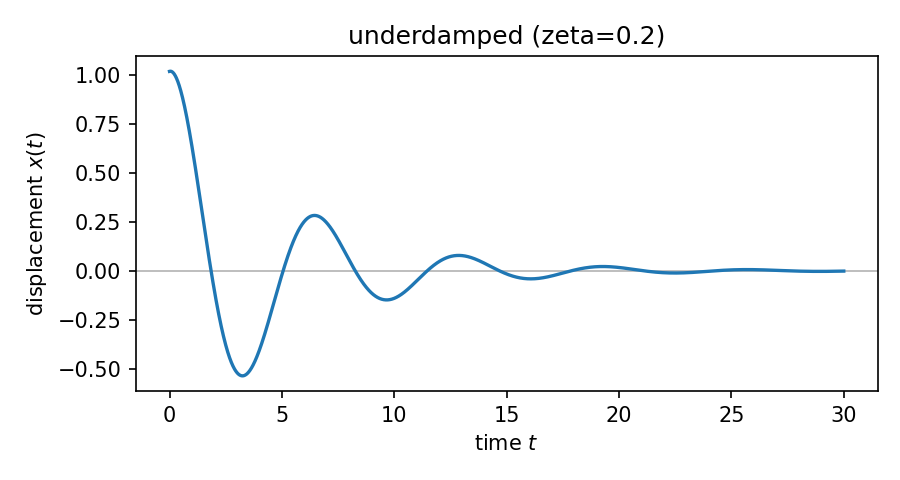
\includegraphics[width=0.72\linewidth]{figures/oscillator_underdamped.png}
  \caption{Underdamped response ($\zeta = 0.2$, $\omega = 1$) from
  \eqref{eq:oscillator}, generated by \texttt{e00001\_damped\_oscillator}
  (campaign~AA) and copied into this note.}
  \label{fig:underdamped}
\end{figure}
